\section{Suite exacte de Pimsner-Voiculescu}
\subsection{La preuve originale}

Maintenant que le décor est planté, nous pouvons passer à la $K$-théorie. 
On pose :  \[d : \left\{\begin{array}{rcl}A & \rightarrow & \mathcal T \\ a & \mapsto & a\otimes I\end{array}\right.\]
Nous allons d'abord démontré le :

\begin{lem}\label{diagramme}
Les diagrammes suivant :
\[\begin{tikzcd}[column sep = huge]
K_i(A\otimes K) \arrow{r}{\psi_*}& K_i(\mathcal T) \\
K_i(A)   \arrow{u}{\simeq}\arrow{r}{(id_A)_*-\alpha(-1)_*}& K_i(A) \arrow{u}{d_*}
\end{tikzcd}
\]
sont commutatifs pour $i\in\{0,1\}$ , et $d_* : K_1(A)\rightarrow K_1(\mathcal T)$ est injectif.
\end{lem}

\begin{dem}
L'isomorphisme $K_1(A)\rightarrow K_1(A\otimes\K)$ associe à une classe $[v]\in K_1(A)$ l'élément $[v\otimes e_{00}+(I-1\otimes e_{00})]$, dont l'image par $\psi_*$ est :
\begin{equation}\label{identite}\psi_*[v\otimes e_{00}+(I-1\otimes e_{00})]= [v\otimes P]+[1\otimes I-1\otimes P] = [v\otimes P]+[1\otimes SS^*]\end{equation}

Maintenant :
\begin{equation}\label{calcul}d_*\circ \left(id_A-\alpha(-1)\right)_*[v]= [ v\otimes I]-[ u^*vu\otimes I]\end{equation}

Soit l'unitaire :\quad\[\Omega = \begin{pmatrix}u\otimes S & Q \\ 0 & u^*\otimes S^*\end{pmatrix}\in \mathcal T \otimes M_2\]

On remarque que :
\[\Omega\begin{pmatrix}u^*vu\otimes I & 0 \\ 0 & 1\otimes I\end{pmatrix}\Omega^*= \begin{pmatrix}v\otimes SS^* +QQ^*& Q(u\otimes S) \\ (u^*\otimes S^*)Q^* & 1\otimes I\end{pmatrix}\]
\[=\begin{pmatrix}v\otimes SS^* +QQ^*& 0 \\ 0 & 1\otimes I\end{pmatrix}\]


Mais la classe dans $K_1$ est invariante par augmentation, i.e. $[x]=\left[\begin{pmatrix}x& 0 \\ 0 & 1\end{pmatrix}\right]$, et par conjugaison par un unitaire, donc :
\[\left[\Omega\begin{pmatrix}u^*vu\otimes I & 0 \\ 0 & 1\otimes I\end{pmatrix}\Omega^*\right]=\left[u^*vu\otimes I\right]\]
En remplaçant dans ~\eqref{calcul}, on obtient :
\begin{align*}
[ v\otimes I]-[v\otimes SS^* +Q]& =[( v\otimes I)(v\otimes SS^* +Q)^{-1}]\\\
&=[v^*\otimes SS^* +Q]\\
&=[1\otimes SS^* +v\otimes P]
\end{align*}

qui est l'expression que l'on avait trouvé pour l'image de $[v]$ par $\psi_*$ dans ~\eqref{identite}. La commutativité du diagramme $i=0$ suit la même preuve : il suffit de remarquer que si l'on prend une projection auto-adjointe $q\in A$, alors dans $K_0(\mathcal T)$ : 
\begin{align*}
[(\alpha(-1)q )\otimes I] & =\left[\Omega\begin{pmatrix}(\alpha(-1)q )\otimes I & 0\\ 0 & 0\end{pmatrix}\Omega^*\right] \\
	& = \left[\begin{pmatrix}q \otimes SS^* & 0\\ 0 & 0\end{pmatrix}\right]\\
	& = [q \otimes SS^*].
\end{align*}
Ceci assure que : \[d_*\circ \left( (id_A)_*-\alpha(-1)_*\right) [q\otimes e_{00}]=[q\otimes I]-[(\alpha(-1)q)\otimes I]=[q\otimes P] =\psi_*[q\otimes e_{00}].\]

Les diagrammes commutent bien, il reste à montrer l'injectivité de $d_*$.\\

Pour cela, montrons que si $v_0$ et $v_1$ sont des unitaires de $A$, et $t\mapsto w_t$ un chemin continu dans les unitaires de $\mathcal T$ d'origine $v_0\otimes I$ et d'arrivée $v_1\otimes I$, alors $[v_0]=[v_1]$ dans $K_1(A)$.\\

Calculons :
\[\begin{pmatrix}w_t & 0 \\ 0 & 1\otimes I\end{pmatrix}\Omega \begin{pmatrix} \tilde{\alpha}(-1)w^*_t & 0 \\ 0 & 1\otimes I\end{pmatrix}\Omega^*
		=\begin{pmatrix}w_t (1\otimes S)w_t^*(1\otimes S^*) + w_t Q& 0 \\ 0 & 1\otimes I\end{pmatrix}.\]

 Le chemin unitaire $y_t=w_t (1\otimes S)w_t^*(1\otimes S^*) + w_t Q\in \mathcal T$ vérifie :
\[\forall t, \quad y_t \in 1\otimes I +J.\]
En effet : 
\[y_t -1\otimes I = (w_t-1\otimes I)Q+w_t\big((1\otimes S)w_t^*-w_t^*(1\otimes S)\big)(1\otimes S^*),\]
mais un élément de la forme $(1\otimes S)w-w(1\otimes S)$ est toujours dans $B\otimes \phi(\K)$, si $w\in \mathcal T$. Si $w$ est dans $A\otimes I$ ou vaut $u\otimes S$, on obtient $0$, et si $w=u^*\otimes S^*$, le commutateur vaut $u^*\otimes P\in B\otimes \phi(\K)$. Ces éléments génèrent un algèbre dense dans $\mathcal T$ : l'assertion en découle.\\

On a donc un chemin continu d'unitaires de $1\otimes SS^*+v_0\otimes P$ à $1\otimes SS^*+v_1\otimes P$, qui reste dans $1\otimes I +J$. Comme $\psi$ établit un isomorphisme de $\C1\otimes I +J$ sur $\tilde{A\otimes \K}$, on a donc, dans $K_1(\tilde{A\otimes \K})$ :
\[[\tilde{I}-1\otimes e_{00}+v_0\otimes e_{00} ]=[ \tilde{I}-1\otimes e_{00}+v_1\otimes e_{00}]\]
donc : $[v_0]=[v_1]$ dans $K_1(A)$, et l'injectivité de $d_*$ est démontrée.
\qed\\
\end{dem}

En passant l'extension de Toeplitz en $K$-théorie, et en combinant avec le lemme \ref{diagramme}, on obtient le diagramme suivant :\\

\begin{tikzcd}[column sep = large]
K_1(A\otimes \K) \arrow{r}{\psi_*} 	& K_1(\mathcal T) \arrow{r}{\pi_*}	& K_1(A\times_\alpha \Z) \arrow{r}{\delta} &K_0(A\otimes \K) \\
K_1(A) \arrow{u}{\simeq} \arrow{r}{(id_A-\alpha(-1))_*}	& K_1(A) \arrow{u}{d_*}	\arrow{ur}{\iota_*}
\end{tikzcd}\\

dont la première ligne est exacte, et le carré commute.\\

\begin{lem}\label{isom} $d_* : K_1(A)\rightarrow K_1(\mathcal T)$ est un isomorphisme.\end{lem} 

\begin{dem}
Montrons que $\text{Ker}\ \delta \subset \text{Im}\ \iota_*$. Cela suffit puisque si $d_*$ n'est pas surjectif, il existe un élément $x\in K_1(\mathcal T)\setminus \text{Im}\ d_*$ , dont l'image par $\pi_*$ n'est pas dans l'image de $\iota_*$. Pourtant : $\delta\circ\pi_*( z) =0$.\\

Nous allons montrer que tout élément de $\text{Ker }\delta$ s'écrit :
\[w=[1\otimes 1_n -F_1+F_1x_1(u^*\otimes 1_n)F_1]_1-[1\otimes 1_n -F_2+F_2x_2(u^*\otimes 1_n)F_2]_1\]
pour certains $x_1$, $x_2$, $F_1$ et $F_2$ dans $A\otimes \frak M_n$ tels que $F_i$ soient des projections auto-adjointes unitairement équivalentes : il existe un unitaire $v\in A\otimes \frak M_n$ les entrelaçant $F_1=vF_2v^*$.\\

Montrons que cela conclut. Dans $K_1(A\times_\alpha \Z)$, on a l'égalité :
\begin{align*}
[1\otimes 1_n -F_2+F_2x_2(u^*\otimes 1_n)F_2]_1 & =[1\otimes 1_n -F_1+F_1 v x_2(u^*\otimes 1_n)v^* F_1]_1 \\
								& = [1\otimes 1_n -F_1+F_1 y (u^*\otimes 1_n)F_1]_1
\end{align*}
où $y=vx_2(\alpha(-1)\otimes id_n)v^*\in A\otimes \frak M_n$. Alors :

\begin{align*}
w & =[\left(1\otimes 1_n -F_1+F_1x_1(u^*\otimes 1_n)F_1\right)\left(1\otimes 1_n -F_1+F_1 y (u^*\otimes 1_n)F_1\right)^*]_1 \\
    & = [1\otimes 1_n -F_1+F_1 x_1 (\alpha(-1)\otimes id_n) F_1 y^* F_1]_1
\end{align*}
L'élément entre crochets est dans $A\otimes \frak M_n$, ce qui veut dire que sa classe $w$ est dans l'image de $\iota_*$ : $\text{Ker}\ \delta \subset \text{Im}\ \iota_*$ est démontré.\\

Montrons maintenat la remarque. Le lemme \ref{generateur} nous permet d'affirmer que tout élément de $K_1(A\times_\alpha \Z)$ s'écrit comme une différence de générateurs unitaires de la forme $[1_n-F+Fx(u^*\otimes 1_n)F]_1$. Si $n=1$, un tel élément a un relevé $w=(1-F)\otimes I+Fxu^*F\otimes S^*\in\mathcal T$. Mais alors :
\begin{align*}
ww^* &=(1-F)\otimes I + Fxu^*Fux^*F\otimes S^*S \\
	&=(1-F)\otimes I +F\otimes I  \\
            & = 1\otimes I  \\
w^*w &=(1-F)\otimes I + Fux^*Fu^*xF\otimes SS^* \\
	&=(1-F)\otimes I +F\otimes (I-P)\\
           & = 1\otimes I-F\otimes P
\end{align*}
L'index est donc facilement calculable :
\begin{align*}\delta[1_n-F+Fx(u^*\otimes 1_n)F]_1 & =[1\otimes I -w^*w]_0-[1\otimes I -ww^*]_0 \\
&=[F\otimes P]_0\\
&=[F\otimes e_{00}]_0
\end{align*}

Ce calcul assure que \[[1_n-F_1+F_1x_1(u^*\otimes 1_n)F_1]_1-[1_m-F_2+F_2x_2(u^*\otimes 1_m)F_2]_1\in \text{Ker }\delta\]
\[ \text{ssi}\quad[F_1]_0=[F_2]_0\quad \text{dans } K_0(A).\]

Quitte à remplacer $F_i$ et $x_i$ par $0_p \oplus F_i$ et $I_p\oplus x_i$, on peut supposer $m=n$. De même, quitte à remplacer $F_i$ et $x_i$ par $F_i\oplus 1\otimes 1_p$ et $x_i\oplus 1\otimes 1_{n+p}$, on peut supposer que $F_1$ et $F_2$ sont unitairement équivalentes.\\
\qed
\end{dem}
On a donc montré que $d_*$ induisait un isomorphisme en $K_1$-théorie. On obtient donc une suite exacte à $6$ termes à partir de l'extension de Toeplitz, dont on voudrait déduire le théorème, ce que l'on peut faire à condition de montrer que $d_*$ induit un isomorphisme au niveau des $K_0$-groupes.\\

\begin{lem}\label{isom} $d_* : K_0(A)\rightarrow K_0(\mathcal T)$ est un isomorphisme.\end{lem} 
\begin{dem}
La suite exacte \begin{tikzcd}[column sep=small]0\arrow{r}& SA\arrow{r}&C(A\otimes \mathbb S^1)\arrow{r}&A\arrow{r}&0\end{tikzcd} est scindée, et induit, modulo la périodicité de Bott, le diagramme commutatif suivant :
\[
\begin{tikzcd}[column sep=small] K_1(A)\arrow{r}& K_0\left( C(A\otimes \mathbb S^1)\right)\arrow{r}&K_0(A)\arrow{d}\\
					K_0(A)\arrow{u}& K_1\left( C(A\otimes \mathbb S^1)\right) \arrow{l}&K_1(A) \arrow{l}
\end{tikzcd} .
\]
Mais, la suite étant scindée, tout élément de $K_i(A)$ se relève, et les flèches connectantes, qui mesurent l'obstruction à être relevé, sont donc nulles : on obtient deux suites exactes scindées :
\[\begin{tikzcd}[column sep=small] 0\arrow{r}& K_{1-i}(A)\arrow{r}& K_i\left( C(A\otimes \mathbb S^1)\right)\arrow{r}&K_i(A)\arrow{r}&0\end{tikzcd} \]
et donc $K_i\left( C(A\otimes \mathbb S^1)\right)\simeq K_0(A)\oplus K_1(A)$.\\

Si on note $\phi^A : SA\oplus A \rightarrow A\otimes C(\mathbb S^1)$ l'isomorphisme obtenu à partir des suites exactes scindées, alors :
\begin{equation}\label{rmq}
(id_{ C(\mathbb S^1)}\otimes d )_*\circ \phi^A_*=\phi^{\mathcal T}_*\circ d_*.
\end{equation} 
Le lemme \ref{isom} appliqué à $id_{ C(\mathbb S^1)}\otimes d  : A\otimes C(\mathbb S^1)\rightarrow \mathcal T(A\otimes C(\mathbb S^1))$, et le fait que $\mathcal T(A\otimes C(\mathbb S^1))=\mathcal T(A)\otimes C(\mathbb S^1)$, assurent que $(id_{ C(\mathbb S^1)}\otimes d )_*$ établit un isomorphisme de $K_1(A\otimes C(\mathbb S^1))$ sur $K_1(\mathcal T \otimes C(\mathbb S^1))$, ce qui, avec la remarque \eqref{rmq} conclut.\\
\qed

\end{dem}
Le théorème \ref{PV} découle directement des lemmes précédents : on passe l'extension de Toeplitz en $K$-théorie et on se sert de la stabilité $K_i(A\otimes \K)\simeq K_i(A)$ et de l'isomorphisme $K_i(A)\simeq K_i(\mathcal T)$.

%%%%%%%%%%%%%%%%%%%%%%%%%%%%%%%%%%%%%%%%%%%%%%%%%%%%%%%%%%%%%%%%%%%%%%%%%%%%%%%%%%%%%%%%%
%%%%%%%%%%%%%%%%%%%%%%%%%%%%%%%%%%%%%%%%%%%%%%%%%%%%%%%%%%%%%%%%%%%%%%%%%%%%%%%%%%%%%%%%%%
\subsection{Un exemple : le tore non-commutatif}
 
Si on se fixe un automorphisme $\alpha \in Aut(A)$, on peut construire le produit croisé $A\times_\alpha \Z$ comme la $C^*$-algèbre universelle engendrée par $A$ et un unitaire $u$ vérifiant :
\[\forall a \in A, uau^*=\alpha(a).\]
Pour la construire effectivement, considérons $A[u]$. La relation de commutation nous donne le produit suivant :
\[au^n bu^m = a \alpha^n(b)u^{n+m}\quad \forall a,b \in A, \forall n,m \in \Z\]
Avec $A=C(\mathbb S^1)$ et $\alpha$ l'automorphisme induit par $z\mapsto e^{2i\pi\theta z}$, on obtient le tore non-commutatif $A_\theta$. Le chemin $\phi_t: z\mapsto e^{2it\pi\theta z}$ montre que $\alpha$ est homotope à l'identité et la suite exacte de Pimsner-Voiculescu se transforme alors en :
\[\begin{tikzcd}
 K_0(C(\mathbb S^1)) \arrow{r}{0} & K_0(C(\mathbb S^1))  \arrow{r}{\iota_*}  &    K_0(A_\theta)  \arrow{d}  \\
 K_1(A_\theta) \arrow{u} & K_1(C(\mathbb S^1))  \arrow{l}{\iota_*} &    K_1(C(\mathbb S^1)) \arrow{l}{0}.
\end{tikzcd}\]

Mais $K_i(C(\mathbb S^1))=K_i(S\C \oplus \C)=K_{1-i}(\C)\oplus K_i(\C)=\Z$, d'où : $K_i(A_\theta)=\Z \oplus\Z, i=0,1$. Nous avons donc calculé les groupes de $K$-théorie du tore non-commutatif, mais nous allons dire plus. On peut en effet calculer les générateurs de ces groupes. \\

\begin{definition}
Un projecteur de Rieffel de $A\times_\alpha \Z$ est un idemptotent autoadjoint de la forme $x_0+x_1 u +u^*x_1^*$, où $x_0,x_1 \in A$.\\
\end{definition}
Un projecteur de Rieffel étant autoadjoint, nous pouvons immédiatement en déduire que $x_0$ aussi. L'idempotence conduit elle au trois relations suivantes : %changer les items
\begin{itemize}
\item $x_0=x_0^2+\alpha^{-1}(x_1^* x_1)+x_1 x_1^*$
\item $x_1= x_0 x_1 +x_1 \alpha(x_0)$
\item $0=\alpha^{-1}(x_1)x_1$.
\end{itemize}

Rappelons que l'algèbre de Von Neumann enveloppante d'une $C^*$-algèbre $A$ est défnie par le bicommutant dans $\mathcal L(H_u)$ de $\pi_u(A)$, où $\pi_u : A\rightarrow \mathcal L(H_u)$ est la représentation universelle de $A$, c'est-à-dire la somme hilbertienne de toutes les représentations irréductibles de $A$.

\begin{definition}
Soit $x\in A$ un élément d'une $C^*$-algèbre.\\
 Le support à gauche de $x$ est défini comme le projecteur orthogonal de $\mathcal L(H_u)$ sur la fermeture de l'image de $\pi_u(x)$. On le note $l_x$.\\
  Le support à droite de $x$ est défini comme le projecteur orthogonal de $\mathcal L(H_u)$ sur l'orthogonal du noyau de $\pi_u(x)$. On le note $r_x$.
\end{definition}
 
Ces deux projecteurs vérifient : $l_x x =x = x r_x, \forall x \in A$ et si $x$ est autoadjoint, alors ils sont égaux.\\

\begin{prop}
Soit $p=x_0+x_1 u +u^*x_1^*\in A\times_\alpha \Z$ une projection de Rieffel et $\Delta := l_{x_1}$ le support à gauche de $x_1$. Alors l'unitaire $\exp(2i\pi x_0 \Delta)$ est dans $A$ et :
\[\delta [p]_0=[\exp(2i\pi x_0 \Delta)]_1.\] 
\end{prop}

\begin{dem}
Soit $p=x_0+x_1 u +u^*x_1^*\in A\times_\alpha \Z $ une projection de Rieffel. Montrons par récurrence que le relevé autoadjoint $a=u^*x_1^*\otimes S^*+x_0\otimes I +x_1 u\otimes S\in \mathcal T$ de $p$ vérifie :
\[\forall n \geq 1, \quad a^n = a+(x_0^n-x_0)\Delta\otimes P.\]
Si c'est vrai au rang $n$,\\
\begin{align*}
a^{n+1} &=a^2+a(x_0^n-x_0)\Delta\otimes P \\
		& =a+a(x_0^2-x_0)\Delta\otimes P+x_0(x_0^n-x_0)\Delta\otimes P+x_1u(x_0^n-x_0)\Delta\otimes SP \\
		& = a+(x_0^{n+1}-x_0)\Delta\otimes P+ u(\alpha(-1)x_1)(x_0^n-x_0)\Delta\otimes SP\\
\end{align*}

Le dernier terme étant nul ($SP=0$), le principe de récurrence conclut.\\

Ayant exhibé un relevé autoadjoint de $p$, on est en mesure de calculer son indice. Mais :
\begin{align*}
\exp(2i\pi a ) &=1\otimes I+\sum_{n\geq 1}\frac{1}{n!}( a+(x_0^n-x_0)\Delta\otimes P)\\
		& = (e^{2i\pi}-1)(a-x_0\Delta \otimes P)+\exp(2i\pi x_0\Delta)\otimes P + 1\otimes (I-P)\\
		& =\psi\left(\exp(2i\pi x_0\Delta)\otimes e_{00} + 1\otimes (I-e_{00})\right).\\
\end{align*}
Il vient : 
\[\partial [p]_0=\left[\exp(2i\pi a )]_1=[\exp(2i\pi x_0\Delta)\otimes e_{00} + 1\otimes (I-e_{00}) \right]_1\]
Le $*$-homomorphisme $\delta$ étant la composition du connectant $\partial : K_0(A\times_\alpha \Z)\rightarrow K_1(A\times \K)$ avec l'isomorphisme $K_1(A\times \K)\simeq K_1(A)$, on en déduit :
\[\delta[p]_0=[\exp(2i\pi x_0\Delta)]_1.\]
\qed
\end{dem}

Ce résultat met à notre disposition une autre méthode de calcul de l'image par l'application exponentielle d'un projecteur dans le cas des projecteur de Rieffel. Il est à rapprocher de la proposition \ref{exp} : Pimsner et Voiculescu ~\cite{PV} décrivent de manière effective l'application exponentielle dans le cas d'un produit croisé $A\times _\alpha \Z$.\\

Nous avons vu que la suite exacte à $6$ termes donnait deux suites exactes courtes, dont :
\[\begin{tikzcd}[column sep = small]0\arrow{r} & K_0(C(\mathbb S^1))\arrow{r}& K_0(A_\theta)\arrow{r}{\delta} & K_1(C(\mathbb S^1)))\arrow{r} & 0   \end{tikzcd}\]
On sait que les groupes à gauche et à droite sont tous les deux $\Z$, l'un étant généré par la classe de la projection $1\in C(\mathbb S^1)$, l'autre par la classe de l'unitaire $z=id_{\mathbb S^1}\in  C(\mathbb S^1)$. Si l'on trouve un projecteur $p$ tel que $\delta [p]_0=[z]_1$, on peut dire que $K_0(A_\theta)$ est engendré par $[1]_0$ et $[p]_0$.\\

On note $\varphi$ la fonction définie par $\alpha (f) (z) = f(e^{2i\pi\theta}z)=f\circ \varphi (z)$.
Soit $0<\delta<\theta$. Soit $f$ la fonction de $\R$, affine par morceaux et $1$ péridiodique, qui vaut $1$ si $t$ est dans $[\delta, \theta]$, $0$ si $t\in [\theta+\delta,1]$ et est nulle en $0$. On pose : 
\[\left\{ \begin{array}{rl}x_0& =e^{2i\pi f }\\
				x_1 (e^{2i\pi t})&= \sqrt{x_0(1-x_0)} 1_{0<t<\delta}
\end{array}\right.\]  

On vérifie par un simple calcul que $p_\theta=x_0+x_1 u +u^*x_1^*$ définit un projecteur de Rieffel. Maintenant, $g$ étant auto-adjoint, son support gauche et droit coïncide (c'est le support de $g$), et $(x_0\Delta)(e^{2i\pi t}) = \frac{t}{\delta}1_{0<t<\delta}$. Cette fonction est homotope à $z$, et donc la proposition précédente conclut : 
\[\delta [p_\theta]_0= [z]_1.\]

Pour déterminer les générateurs de $K_1(A_\theta)$, observons la suite exacte 
\[\begin{tikzcd}[column sep = small]0\arrow{r} & K_1(C(\mathbb S^1))\arrow{r}& K_1(A_\theta)\arrow{r}{\delta} & K_0(C(\mathbb S^1)))\arrow{r} & 0   \end{tikzcd}.\]
A nouveau, les deux groupes à droite et à gauche sont $\Z$ donc $K_1(A_\theta)$ est un groupe libre abélien à deux générateurs. Le premier est donné gratuitement : on a vu que $K_1(C(\mathbb S^1))$ était généré par la classe de l'inclusion $v: \mathbb S^1 \rightarrow \C$, donc son image dans $K_1(A_\theta)$, c'est à dire $[v]_1$, est un premier générateur. \\
Grâce aux lemmes \ref{generateur} et \ref{isom}, on sait que $K_1(A_\theta)$ est généré par des classes d'unitaires de la forme $[1-F+Fx(u^*\otimes 1_n)]_1$ dont l'indice est 
\[\delta [1-F+Fx(u^*\otimes 1_n)]_1= [F\otimes e_{00}]_0.\]
L'indice de $u^*$ est donc directement calculable :
\[\delta [u^*]_1= [1]_0,\]
et c'est un générateur de $K_0(C(\mathbb S^1))$. Donc $K_1(A_\theta)$ est isomorphe à $\Z$, généré par les classes de $u$ et $v$. Ici $u$ représente l'unitaire qui rend intérieure l'action de $\Z$ sur $C(\mathbb S^1)$, et $A_theta$ est engendrée par les deux unitaires $u$ et $v$ soumis à la relation $u^*vu =e^{2i\pi\theta} v$.\\

Tout élément de $A_\theta$ peut se décomposer en <<série de Fourier>> sous la forme 
\[x=\sum_{n\in \Z}f_n u^n\quad, f_n \in C(\mathbb S^1) \]
avec convergence en norme des séries partielles. Alors $\tau(x):=\int_{\mathbb S^1} f_0(z)\mu(dz)$, où $\mu$ est la mesure de Haar normalisé sur $\mathbb S^1$, définit une trace continue normalisée, qui est fidèle lorsque $\theta$ est irrationnel. Cette trace induit un morphisme $\tau_* : K_0(A_\theta)\rightarrow \C$.\\

Quelques remarques :
\begin{enumerate}
\item On voit que $K_*(A_\theta)=\Z\oplus \Z$, pour tout $\theta$ irrationnel. En particulier les groupes de $K$-théorie ne distinguent pas entre les différentes algèbres de rotation irrationnelles. 
% Quels sont les groupes de Ktheorie de Atheta pour un angle rationel
\item Le résultat précédent permet en particulier de montrer que l'image du morphisme induit $\tau_* : K_0(A_\theta)\rightarrow \C$ est exactement $\Z+\theta \Z$, en calculant $\tau(1)=1$ et $\tau(p_\theta)=\theta$. Ceci a permis à M. Rieffel de montrer dans~\cite{Rieffel} que, si $\theta$ et $\theta'$ sont irrationnels, alors $A_\theta$ et $A_\theta'$ sont isomorphes ssi les parties fractionnaires de $\theta$ et $\theta'$ ou celles de $\theta$ et $1-\theta'$ sont égales.
\end{enumerate}

En guise de conclusion, le lecteur interessé est invité à lire l'article de Pimsner écrit en $1997$, \textit{A class of $C^*$-algebras generalizing both Cuntz-Krieger algebras and crossed products by $\mathbb Z$}~\cite{Pimsner}, qui généralise la suite exacte à six-termes pour les produits croisés. Dans ce papier, Pimsner construit pour tout $A-A$-bimodule hilbertien $E$ deux $C^*$-algèbres $\mathcal O _E$ et $\mathcal T_E$. Il montre alors que lorsque l'on considère $A$ comme bimodule hilbertien sur lui-même, on retrouve $\mathcal O_A = A\times_\alpha \Z$ pour un certain automorphisme $\alpha$. De la même façon que dans~\cite{PV}, il prouve une $K$-équivalence entre $\mathcal T _E$ et $A$, et en déduit des suites exactes à six-termes en $KK$-théorie.\\

Côté applications, le tore non-commutatif apparaît dans des modèles appelés modèles de Harper, dont l'objectif est de décrire un électron se déplaçant dans un réseau cristallin soumi à un champ magnétique uniforme :  l'électron se déplace dans un solide constitué de noyaux immobiles positionnés aux noeuds du réseau. Par exemple, on peut considérer le réseau $\Z^2$ sur lequel on applique un champ magnétique perpendiculaire constant, dont le flux normalisé est $2\pi\alpha=2\pi \frac{\phi}{\phi_0}$, $\phi_0=\hbar/e$ étant le quantum de flux et $\phi$ le flux par maille. L'espace de Hilbert naturellement associée à ce problème est $l^2(\Z^2)$, et on considère alors l'algèbre d'opérateurs définis par
\[W(m)\psi(x) = e^{i\pi \alpha \{x,m\} }\psi(x-m)\quad, \forall m,x\in \Z^2,\psi\in l^2(\Z^2) \]
où $\{x,m\}=x_1 m_2 -x_2 m_1$.\\

En posant $U_1=W(1,0)$ et $U_2=W(0,1)$, tout opérateur s'écrit 
\[W(m)=U_1^{m_1}U_2^{m_2}e^{i\pi\alpha m_1 m_2}\]
et $U_1$ et $U_2$ vérifient la relation $U_1 U_2 = e^{2i\pi \alpha}U_2 U_1$ : on reconnaît $A_{2\pi\alpha}$. Or les physiciens affirment que l'opérateur hamiltonien du système étudié, dont le spectre donne les valeurs possibles de l'énergie, est l'opérateur de Harper :
\[H_\alpha = U_1+U_1^*+U_2+U_2^*.\]
On peut montrer qu'en un certain sens, le spectre est continu en $\alpha$. Si le flux $\alpha=\frac{p}{q}$ est rationnel, le spectre est séparé en $q$ bandes. Pour les valeurs irrationnelles du flux, le spectre est un ensemble de Cantor, c'est-à-dire un fermé nulle part dense sans point isolé. Pour plus de détails, on pourra se reporter au séminaire Bourbaki de J. Bellissard \cite{Bellissard}. Pour en avoir une idée, on peut observer numériquement les valeurs du spectre pour les rationnels. Il suffit pour cela de calculer le spectre de matrices de dimensions finies grâce à la représentation fidèle de $A_{2\pi \frac{p}{q}}$
\[\pi(U_1)=\begin{pmatrix}0 & 1 & 0 ... & 0 &0\\
0& 0 &1 ... & 0 & 0 \\
. & . & .      & . & . \\
0 & 0 & 0... & 0 & 1 \\
1 & 0 &0 ... & 0& 0 
\end{pmatrix}\in M_q(\C),\quad \pi(U_2)=\text{diag}\left(e^{2i\pi (j-1)\frac{p}{q}}\right)_{j=1,q}.\]
On obtient alors ce que l'on appelle le papillon de Hoftstadter i.e. l'ensemble $\{(x,\alpha) : \alpha \in ]0,1[, x\in Spec(H_\alpha)\}$ du plan. Voici une image générée avec Scilab.

\begin{figure}[h]\centering
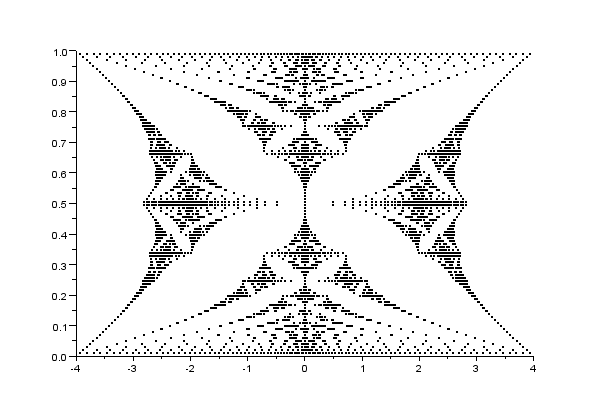
\includegraphics[scale=0.6]{Hofstadter.png}
\caption{Papillon de Hofstadter}
\label{fig:Hoftstadter}
\end{figure}